\documentclass[14pt]{extreport}
\usepackage[paper=a4paper,top=2cm,left=2cm,right=2cm,
    footskip=1cm,bottom=2cm]{geometry}

\usepackage{times}
\usepackage[T1]{fontenc}
\usepackage[utf8]{inputenc}
\usepackage[english,russian]{babel}
\usepackage{amssymb,amsfonts,amsmath,mathtext,amsbsy}
\usepackage{multirow}
\usepackage{listings, color}
\usepackage{graphicx}
\usepackage{import}
\graphicspath{{images/}}

\renewcommand{\baselinestretch}{1.25}
\newcommand{\comment}[1]{}
\newcommand{\br}[1]{\boldsymbol{\mathrm{#1}}}
\renewcommand{\vec}[1]{\br{#1}}
\newcommand{\att}{\text{att}}
\newcommand{\abinom}[2]{\genfrac{}{}{0pt}{0}{#1}{#2}}

\DeclareMathOperator{\rot}{rot}
\newcommand{\Reyn}{\text{Re}}
\newcommand{\Pran}{\text{Pr}}
\newcommand{\Nuss}{\text{Nu}}

%\newcommand{\br}[1]{\bm{\mathrm{#1}}}

\newenvironment{packed_enum}{
\begin{enumerate}
  \setlength{\itemsep}{1pt}
  \setlength{\parskip}{0pt}
  \setlength{\parsep}{0pt}
}{\end{enumerate}}

\newenvironment{packed_itemize}{
\begin{itemize}
  \setlength{\itemsep}{1pt}
  \setlength{\parskip}{0pt}
  \setlength{\parsep}{0pt}
}{\end{itemize}}

\title{VVHD}
\author{Я. А. Дынников}

\begin{document}

%\lipsum[1-2]
\maketitle

%%%%%%%%%%%%%%%%%%%%%%%%%%%%%%%%%%%%%%%%%%%%%%%%%%%%%%%%%%%%%%%%%%%%%%%%%%%%%%%%
\begin{abstract}
Это мануал, посвященный исходникам библиотеки. Здесь я постараюсь 
описать его структуру, способы работы с ним, и подводные камни, 
на которые нужно будет обращать внимание.
\end{abstract}

\chapter{VVHDFlow}

\section{TVec}
Представляет собой структуру из двух double: rx, ry.
Поддерживает основные операторы, сложение, умножение, деление на число итд.
Отдельно стоит упомянуть оператор rotl(TVec $\br r$) - поворот вектора влево на $90^{\circ}$. В математических терминах он эквивалентен $\br e_z \times \br r$.

Есть еще одна хитрость, связанная с векторным умножением. Так как пространство у нас двумерное, то векторное произведение двух векторов нашему пространству не принадлежит, и сохраняем мы от него только модуль: double c = rotl(a)*b;

\begin{equation*}
[\br a \times \br b] = \left|\begin{array}{ccc}
\br e_x & \br e_y & \br e_z \\
a_x & a_y & 0 \\
b_x & b_y & 0 \end{array}\right| = \br e_z \cdot (a_x b_y - a_y b_x) = \br e_z \cdot \binom{-a_y}{a_x} \cdot \binom{b_x}{b_y} = \br e_z \cdot \left( [\br e_z \times \br a] \cdot \br b \right)
\end{equation*}

\section{TObj}
Дочерний класс TVec с лишними компонентами величины (double g), скорости, и запасной переменной double \_1\_eps. TObj используется для почти всех частиц: вихревых, тепловых, меченых. В переменной g у каждого типа хранится свое значение. Для вихревых доменов это циркуляция $\gamma$; для тепловых --- интенсивность $q = \int TdS$; для меченых частиц --- просто номер маркера. Переменная \_1\_eps чаще всего используется для хранения диффузионного эпсилон (расстояние до второго ближайшего объекта), хотя в утилитах ей находятся и другие применения.

\section{TList}
Лист является шаблонным классом и надстройкой над массивом. 
Лист предоставляет функции добавления, удаления элементов и 
динамического изменения размеров. В принципе, лист является 
усовершенствованным вектором (из std::), он даже почти полностью
с ним совместим.

\lstset{language=C++, frame=single, keywordstyle=\color{blue}, morekeywords={size_t}}
\begin{lstlisting}
template <class T>
class list
{
	public:
		list();
		~list();

		void push_back(const T &item);
		void erase(T* item);
		void clear();
		T& at(size_t i);
		T* begin();
		T* end();
		size_t size();
		size_t size_safe();
		T* next(T* item);
		T* prev(T* item);

	private:
		size_t size_;
		size_t maxsize;
		T* begin_;
		T* end_;

		void realloc_();
};

#define const_for(list, it) \
	for (auto it=list->begin(); it<list->end(); it++)
\end{lstlisting}

Вот о чем нужно помнить
\begin{enumerate}
\item Если вы добавляете в массив элементы, не пользуйтесь 
инкрементом TObj* obj++. Если вдруг произойдет realloc ---
адресация массива сменится непредсказуемо.
\item При удалении элемента на его место перемещается последний 
элемент, а size уменьшается.
Если Вы удалили элемент функцией erase(), не забудте указатель
уменьшить на единичку, иначе этот элемент массива останется необработанным
\end{enumerate}

%%%%%%%%%%%%%%%%%%%%%%%%%%%%%%%%%%%%%%%%%%%%%%%%%%%%%%%%%%%%%%%%%%%%%%%%%%%%%%%%
\section{Обозначения}
\label{notations}
Сейчас попробуем ввести индексы для каждого массива, так что бы в формулах не происходило путаницы.
\begin{packed_itemize}
\item $v$ --- индекс свободных вихрей. Их количество $N_v$
\item $h$ --- индекс тепловых частиц. Аналогично количество $N_h$
\item $b$ --- индекс тела. Количество тел = $N_b$
\item $s$ --- индекс отрезков на теле. Так как тел много, то примеяется вместе с $b$. $N_{sb}$ --- число отрезков на $b$-ом теле.
\item $m$ --- индекс меченых часиц (маркеров).
\item $i$ --- запасной индекс. Например для нумерации сенсоров в пространстве.
\end{packed_itemize}

%%%%%%%%%%%%%%%%%%%%%%%%%%%%%%%%%%%%%%%%%%%%%%%%%%%%%%%%%%%%%%%%%%%%%%%%%%%%%%%%
\section{Reference frame}
\label{refframe}
Расчет проводится в системе координат, ни с чем не связанной. Это значит что в этой системе у каждого объекта есть своя скорость. В отличие от предыдущей версии программы, где система отсчета была жестко связана с телом, а пересчет в другую СО проводился уже при постобработке, в данной версии тела представляются закрепленными на пружине к державке, которая имеет свою детерминированную скорость.

Таким образом у нас есть богатый выбор переменных:
\begin{packed_itemize}
\item $\br V_\infty(t)$ --- скорость жидкости на бесконечности.
\item $\Gamma_{\infty}$ --- циркуляция на бесконечности. Константа. Моделирует вихрь, ушедший на бесконечность. Эта переменная пригодится нам для расчета вращающегося цилиндра и аэродинамических профилей.
\item $\br V_b(t)$, $\omega_b(t)$ --- Скорость державки $b$-го тела. Поступательная и вращательная.
\item $\br V_{b?}$, $\omega_{b?}$ --- Полная скорость тела, (включает скорость державки относительно системы координат + скорость тела относительно державки). Подробнее об этом в секции~\ref{tbody}
\end{packed_itemize}

\comment{Система координат используется правая. Это значит, если вы рисуете ось $Ox$ слева на право, а ось $Oy$ снизу вверх, то положительным направлением вращения будет являться вращение против часовой стрелки.

Помимо основной системы координат, имеется так же система координат тела: $Ox_b y_b$. С основной системой координат она связана выражением
\begin{equation*}
\br r = \br r_c + \left(\begin{array}{cc}
\cos(\alpha) & -\sin(\alpha) \\
sin(\alpha) & \cos(\alpha) \end{array}\right) \cdot \br r_b
\end{equation*}
Центр поворота жестко связан с центром системы $Ox_b y_b$. Это нужно учитывать при загрузке тела. Система осчета тела используется только при загрузке. Везде внутри комплекса координаты тела записываются в основной системе. 
\begin{center}\input{RefFrames.pdf_tex}\end{center}
}

%%%%%%%%%%%%%%%%%%%%%%%%%%%%%%%%%%%%%%%%%%%%%%%%%%%%%%%%%%%%%%%%%%%%%%%%%%%%%%%%
\section{Discrete view}
\label{tbody}

Файл body.h описывает класс \textbf{TBody}, в котором хранится тело.
Поверхность тела представляет собой массив отрезков класса \textbf{TAtt} (наследник TObj
\footnote{Это сделано из-за того, что дерево работает с классом TObj*. Тем не менее одно неудобство остается: при получении отрезка из дерева тип все равно придется приводить к TAtt* руками.}).\\

Основные переменные в классе TAtt:
\begin{packed_itemize}
\item $\vec r$ --- координаты центра
\item $\gamma$ --- неизвестная циркуляция (располагается в центре отрезка)
\item $\vec c$ --- вектор начала отрезка
\item $\Delta \vec l$ --- вектор отрезка. При обходе жидкость слева
\item $q_\att$ --- интенсивность присоединенного источнка
\item $\gamma_\att$ --- циркуляция присоединенного вихря
%\item gsum --- суммарная интенсивность, рожденная на данном отрезке на данном шаге
%\item hsum --- суммарная тепловая энергия, подробности потом уточню %TODO
%\item fric --- для хранения вклада в трение
\end{packed_itemize}

Как уже говорилось в секции~\ref{refframe}, комплекс моделирует тело, закрепленное на пружине. Пружина, в свою очередь, крепится к виртуальной ``державке'', которая фиксирует все 3 степени свободы: 2 поступательные, и 1 вращательную.
В программном комплексе хранятся две скорости: скорость державки и скорость тела. Обе скорости записаны относительно основной системы отсчета. Державка движется со скоростью $\vec V_b(t)$, $\omega_b(t)$. Эта скорость детерминирована, ее пользователь задает при запуске программы. Полная скорость движения тела находится из СЛАУ и обозначается через $\vec V_{b?}$, $\omega_{b?}$. Скорость движения тела относительно державки легко угадать: $(\vec V_{b?} - \vec V_b)$, $(\omega_{b?} - \omega_b)$. Для сохранения координат державки и тела в классе TBody имеются специальные переменные: 

\begin{packed_itemize}
\item $\alpha$ --- угол поворота державки относительно основной системы координат
\item $\vec R$ --- смещение державки относительно начала системы координат
\item $\Delta \alpha$ --- поворот тела отительно державки (поворот пружины)
\item $\Delta \vec R$ --- смещение тела относительно державки (растяжение пружины)
\end{packed_itemize}

Функции getRotation, setRotation, getMotion, setMotion манипуляруют с детерминированной скоростью тела (точнее державки), угловой и поступательной.
Функции doRotation, doMotion принимают в качестве аргумента величины ($\vec V_{b?} \Delta t$), ($\omega_{b?} \Delta t$). Изменения, которые они вносят, описываются следующими формулами:\\
$\alpha = \alpha + \omega \cdot \Delta t$\\
$\vec R = \vec R + \vec V \cdot \Delta t$\\
$\Delta \alpha = \Delta \alpha + (\omega_{?} - \omega) \cdot \Delta t$\\
$\Delta \vec R = \Delta \vec R + (\vec V_{?} - \vec V) \cdot \Delta t$\\

Помимо изменений общих координат, изменяются все углы тела, вектора отрезков и координаты центров. Как следует из формул, порядок выполнения поворота или сдвига значения не имеет.
\begin{equation*}
\begin{split}
\vec c_s \vert_\text{Rotation}
& = (\vec R + \Delta \vec R) +
\begin{pmatrix}
\cos & -\sin \\ \sin & \cos
\end{pmatrix}
(\omega_? \Delta t) \cdot \underbrace{(\vec c_s - (\vec R + \Delta \vec R))}_{\vec c_*}\\
& = (\vec R + \Delta \vec R) + \vec c_* \cos(\omega_? \Delta t) + [\vec e_z \times \vec c_*] \sin(\omega_? \Delta t)
\\ \vec c_s \vert_\text{Motion} &= \vec c_s + \vec V_? \Delta t
\end{split}
\end{equation*}

Для моделирования двигающегося тела используется понятие присоединенных вихрей и источников. Они располагаются в центре каждого отрезка и имитируют разрыв скорости на поверхности. %FIXME I need help.
Интенсивность присоединенного источника и циркуляция присоединенного вихря зависят от скорости отрезка, к которому они привязаны.
\begin{equation}
\label{eq_SegmentVelocity}
\vec V_s = \vec V_? + \omega_? \cdot [\vec e_z \times \underbrace{(\vec r_s - (\vec R + \Delta \vec R))}_{r_*}],
\end{equation}
где $\lbrace\vec R + \Delta \vec R\rbrace_b$ --- ось вращения данного тела\footnote{Заметьте, осью вращения является не державка, а место крепления пружины к телу.}. Здесь сделано предположение о малости отрезка и об однородности скорости по всей длине. В таком случае формулы для вычисления присоединенной циркуляции и интенсивности будут иметь вид.
\begin{equation}
\label{eq_AttachIntensity}
\begin{split}
\gamma_{\att~s} &= -\vec V_s \cdot \Delta \vec l_s  = \vec n \times \vec V_s\\
q_{\att~s} &= -[\vec V_s \times \Delta \vec l_s] = \vec n \cdot \vec V_s\\
\end{split}
\end{equation}

Присоединенные вихреисточники должны учитываться при вычислении конвективной скорости, при вычислении давления, при заполнении СЛАУ.
Если расписать формулы~\ref{eq_AttachIntensity} с учетом~\ref{eq_SegmentVelocity}, то получится
\begin{equation}
\label{eq_AttachIntensityLong}
\begin{split}
\gamma_{\att~s} &=
-V_{?x} \cdot (\Delta l_{sx}) - V_{?y} \cdot (\Delta l_{sy}) - \omega_? \cdot [\Delta \vec l_s \times \vec r_*]\\
q_{\att~s} &=
-V_{?x} \cdot (\Delta l_{sy}) + V_{?y} \cdot (\Delta l_{sx}) + \omega_? \cdot (\Delta \vec l_s \cdot \vec r_*)\\
\end{split}
\end{equation}

%%%%%%%%%%%%%%%%%%%%%%%%%%%%%%%%%%%%%%%%%%%%%%%%%%%%%%%%%%%%%%%%%%%%%%%%%%%%%%%%
\section{Geometry formulae}
В будущем нам так-же понадобятся формулы вычисления центра масс, площади и момента инерции тела. Привожу их здесь.

Площадь легче всего вычислить как сумму площадей трапеций $S_\text{body} = \sum S_\text{att~i}$. Для трапеции используем формулу полусумма оснований на высоту. $S_i = \frac{1}{2}(x_{i+1}-x_i)(y_i+y_{i+1})$
Здесь стоит сказать пару слов про обход контура. Положительным направлением обхода считается направление, при котором жидкость находится по левую руку. То есть если вы загрузили тело, обход которого совершается по часовой стрелке (ось абсцис направлена вправо, ординат --- вверх) --- вы получите внешнее обтекание. Если загруженное тело составлено против часовой стрелки --- течение внутри замкнутой области. Для внутренних течений площадь тела, вычисленная по этой формуле окажется отрицательной (как и момент инерции). Это нужно будет учитывать в будущем, а пока мы не занимаемся течениями в канале, можно расслабиться.

Для вычисления центра масс удобно использовать формулу Грина. Но я спер эту формулу из википедии
\begin{equation*}
\vec r_\text{com}
= \dfrac{1}{S}\int \vec r dS
= -\dfrac{1}{3S}\sum_s \vec r_s [\vec c_{s} \times \vec c_{s+1}]
\end{equation*}

Эта формула для момента инерции тоже из вики.
\begin{equation*}
J_0 = \int r^2 dS =
-\dfrac{1}{12} \sum 
\left(
	c_i^2 + \vec c_i \vec c_{i+1} + c_{i+1}^2
\right) \cdot [\vec c_i \times \vec c_{i+1}]
\end{equation*}

Это не совсем момент инерции, так как в него не входи плотность. Он обезразмерен на плотность жидкости, как и все уравнения, которые мы решаем. Поэтому во всех последующих выкладках для сил перед этим самым моментом будет появляться отношение $\rho_b/\rho_0$.
Этот момент инерции вычислен относительно центра основной системы координат. Пересчитать его относительно центра масс или оси вращения легко: $J_\text{com} = J_0 - S r_\text{com}^2$, $J_c = J_\text{com} + S (r_c - r_\text{com})^2$

%%%%%%%%%%%%%%%%%%%%%%%%%%%%%%%%%%%%%%%%%%%%%%%%%%%%%%%%%%%%%%%%%%%%%%%%%%%%%%%%
\section{Convective}
\subsection{Конвективная скорость}
Скорость, индуцированная вихрем $(\vec r_\gamma, \gamma)$ в точке $\vec r$
вычисляется по формуле
\begin{equation}
\label{eq_VortexConvective}
\vec V_\gamma(\vec r) = \frac{1}{2\pi} [\vec e_z \times \vec K(\vec r, \vec r_\gamma)] \cdot \gamma,
\end{equation}
а скорость, индуцированная источником $(\vec r_q, q)$ --- по формуле
\begin{equation}
\label{eq_SourceInfluence}
\vec V_q(\vec r) = \frac{1}{2\pi} \vec K(\vec r, \vec r_q) \cdot q.
\end{equation}


$\br K (\br r, \br r_i)$ можно вычислять несколькми способами:
\begin{packed_enum}
\item Классическая формула для точечного вихря:
$\br K_1 = \dfrac {\Delta\br r}{\Delta r^2}$
, $\Delta \vec r = \vec r - \vec r_i$

\item Для вихря Рэнкина:
$\br K_2 = \begin{cases}
\Delta\br r / r_0^2,	&\Delta r \le r_0 \\
{\Delta\br r}/{\Delta r^2}, 	&\Delta r>r_0\\
\end{cases}$
\\ (круг постоянной завихренности)

\item Для вихря Лэмба:
%TODO Математическая неточность: вихрь Лэмба не согласуется со скоростью источника
$\br K = \br K_3 = \dfrac {\Delta\br r}{\Delta r^2 + \delta^2}$
\end{packed_enum}

Мы пользуемся третьим способом. Эта формула удобнее и быстрее.

%%%%%%%%%%%%%%%%%%%%%%%%%%%%%%%%%%%%%%%%%%%%%%%%%%%%%%%%%%%%%%%%%%%%%%%%%%%%%%%%
\subsection{Flow}
\label{Flow}

Название этой функции сложилось исторически. Она описывает влияние вихревого отрезка на точку, либо наоборот --- вихря на отрезок.
Короче, позволяет аналитически вычислить интеграл

\begin{equation}
\label{eq_Flow}
\begin{split}
\int\limits_{\vec c_1}^{\vec c_2} [\vec e_z \times \vec K_2(\vec r,\vec r_\gamma)] \cdot dr &= \binom{\Re(z_V)}{\Im(z_V)}, \\
z_V &= \begin{cases}
	-i \cdot \log \left(\dfrac{z-z_1}{z-z_2}\right) \cdot \dfrac{|z_2 - z_1|}{z_2 - z_1} \\
	- \left(z - \dfrac{z_1+z_2}{2} \right) \cdot \dfrac{|z_2 - z_1|}{r_0^2} \\
\end{cases}
\end{split}
\end{equation}

$z = (r_{\gamma x}) - i (r_{\gamma y})$, $z_{1,2} = (c_{1,2~x}) - i (c_{1,2~y})$, $z_s = (r_{sx}) - i (r_{sy}) = \frac{1}{2}(z_1 + z_2)$
Если один из концов отрезка является ближним, а другой дальним, 
отрезок делится на две части точкой $z_3$, для каждой
из которых влияние вычисляется по своей формуле.
Такое раздвоение вызвано тем, что под интегралом стоит
функция $\vec K_2$, а не $\vec K_3$: ее удобнее интегрировать.

%%%%%%%%%%%%%%%%%%%%%%%%%%%%%%%%%%%%%%%%%%%%%%%%%%%%%%%%%%%%%%%%%%%%%%%%%%%%%%%%
\subsection{ConvectiveInfluence}
\label{ConvectiveInfluence}
Функция вычисляет интеграл нормальной скорости, индуцируемой единичным вихрем 
в точке $\vec r_\gamma$ на отрезок $[\vec c_1, \vec c_2]$.

\begin{equation}
\label{eq_VortexInfluence}
\begin{split}
\Xi_\gamma(\vec c_1, \vec c_2, \vec r_\gamma)
%%%%%%%%%
&= \frac{1}{2\pi} \int\limits_{\vec c_1}^{\vec c_2} [\vec e_z \times \vec K(\vec r,\vec r_\gamma)] \cdot \vec n \cdot dr
%%%%%%%%%
= \\ &= \frac{1}{2\pi} \cdot
\begin{cases}
-\Re \left\lbrace \log \left(\dfrac{z-z_1}{z-z_2}\right) \right\rbrace,	&\text{для дальних}\\
\dfrac{1}{\varepsilon^2}\Re \left\lbrace (z_s-z)(\bar z_2 - \bar z_1) \right\rbrace, 	&\text{для ближних}\\
\end{cases}
\end{split}
%TODO записать по русски условия
\end{equation}
\begin{center}\input{images/ConvInfluence.pdf_tex}\end{center}

В обычном случае, функцию для блихних вихрей удобней записать без использования
комплексных чисел:
$\frac{1}{2\pi} (\vec r_{sb} - \vec r_v) \Delta\vec l_{sb} / \varepsilon^2$

Аналогичная формула $\Xi_q$ вычисляет влияние единичного источника на отрезок.
\begin{equation}
\label{eq_SourceInfluence}
\begin{split}
\Xi_q (\vec c_1, \vec c_2, \vec r_q)
%%%%%%%%%%
&= \frac{1}{2\pi} \int\limits_{\vec c_1}^{\vec c_2} \vec K(\vec r, \vec r_q) \cdot \vec n \cdot dr
%%%%%%%%%%
= \\ & = -\frac{1}{2\pi} \cdot
\begin{cases}
\Im \left\lbrace \log \left(\dfrac{z-z_1}{z-z_2}\right) \right\rbrace,	&\text{для дальних}\\
\dfrac{1}{\varepsilon^2}\Im \left\lbrace (z_s-z)(\bar z_2 - \bar z_1) \right\rbrace, 	&\text{для ближних}\\
\end{cases}
\end{split}
\end{equation}
Без использования комплексных чисел формула для ближних источников принимает вид
$\frac{1}{2\pi} [\Delta \vec l_{sb} \times (\vec r_{sb} - \vec r_v)]/\varepsilon^2$

%%%%%%%%%%%%%%%%%%%%%%%%%%%%%%%%%%%%%%%%%%%%%%%%%%%%%%%%%%%%%%%%%%%%%%%%%%%%%%%%
\subsection{SegmentInfluence}
\label{SegmentInfluence}

Эти формулы описывают скорость, индуцированную в точке $\vec r_0$ отрезком $[\vec c_1, \vec c_2]$ с линейным распределением источников интенсивностью от $q_1$ до $q_2$. В отличие от предыдущих формул источники здесь точечные.

$z_{12} = (r - r_{12})_x + i (r-r_{12})_y$, $r$ --- точка наблюдения

\begin{equation}
\label{eq_SegmentInfluence_source}
\vec V_{sq} (z_1, z_2, q_1, q_2) = \dfrac{1}{2\pi}  \int_{z_1}^{z_2}\dfrac{q}{z^*} dz = \dfrac{1}{2\pi} \dfrac{1}{(z_2-z_1)^*} \cdot \left(  (q_2-q_1) - \dfrac{q_2 z_1^* - q_1 z_2^*}{(z_2-z_1)^*}\ln \dfrac{z_2^*}{z_1^*} \right)
\end{equation}

%%%%%%%%%%%%%%%%%%%%%%%%%%%%%%%%%%%%%%%%%%%%%%%%%%%%%%%%%%%%%%%%%%%%%%%%%%%%%%%%
\subsection{СЛАУ}

Для вычисления циркуляций новых доменов, на каждом шаге решается система линейных алгебраических уравнений. Составлять ее можно несколькими способами, но в самом общем варианте в нее входит несколько типов условий:

\begin{packed_enum}
\item Условие непротекания/прилипания. Мы используем интегральный вариант
\begin{equation*}
\int{\vec V_\text{liquid}(\vec r) \cdot \vec n \cdot dr} = \int {\vec V_\text{body}(\vec r) \cdot \vec n \cdot dr}
\end{equation*}
Интеграл вычисляется по конткетному отрезку аналитически по формуле~(\ref{ConvectiveInfluence}). $\br V_\text{liquid}$ --- скорость жидкости, которая включает в себя индуцированную свободными и присоединенными вихрями, а так же скорость на бесконечности. $\br V_\text{body}$ --- скорость самого отрезка~(\ref{eq_SegmentVelocity}).
\item Условие отсутствия возмущений на бесконечности. Если говорить кратко, то $\sum \gamma = 0$, что имеено подразумевается под $\gamma$ зависит от конкретного случая; об этом будет рассказано позже.
\item Второй закон Ньютона. $\br F = m \br a$. Более подробно об этом позже.
\end{packed_enum}

Прежде чем расписывать каждое уравнение в отдельности, определимся с тем, что мы ищем. Неизвестными переменными на каждом временном шаге являются циркуляции новых доменов и скорости тела: $\vec V_?$, $\omega_?$. Известными величинами являются скорость и циркуляция на бесконечности ($\vec V_\infty$, $\Gamma_\infty$), скорость державки тела ($\vec V$, $\omega$), коэффициенты упругости пружины ($k_x$, $k_y$, $k_\alpha$). Вектор неизвестных величин составим следующим образом:

\begin{equation}
\label{eq_5_3_1}
X_b =
\left(\begin{matrix}
\gamma_1 & \dotsc & \gamma_{N_s}& ~~V_{?x}& V_{?y}& \omega_?\\
\end{matrix}\right)^T
\end{equation}

Это для одного тела. Если тел несколько --- итоговый вектор будет состоять из нескольких таких частей. Теперь придется подробно расписать каждое уравнение в системе. 

%%%%%%%%%%%%%%%%%%%%%%%%%%%%%%%%%%%%%%%%%%%%%%%%%%%%%%%%%%%%%%%%%%%%%%%%%%%%%%%%
\subsection{Условие непротекания/прилипания}

Говоря русским языком, жидкость не должна протекать внутрь тела. Мы используем интегральный вариант
\begin{equation*}
\int{\vec V_\text{liquid}(\vec r) \cdot \vec n \cdot dr} = \int {\vec V_\text{body}(\vec r) \cdot \vec n \cdot dr}
\end{equation*}
Интеграл вычисляется по конткетному отрезку аналитически по формуле~(\ref{ConvectiveInfluence}). $\br V_\text{liquid}$ --- скорость жидкости, которая включает в себя индуцированную свободными и присоединенными вихрями, а так же скорость на бесконечности. $\br V_\text{body}$ --- скорость самого отрезка~(\ref{eq_SegmentVelocity}).

Расписывая каждое слагаемое в отдельности получим уравнение для отрезка $[\vec c_1, \vec c_2]$

\begin{equation}
\label{eq_noslip}
\left(\begin{matrix}
\Xi_\gamma(\vec c_1, \vec c_2, \vec c_s)\dotsc& ~~a_{I}& a_{II}& a_{III}\\
\end{matrix}\right)
\cdot X
=
-[\Delta \vec l \times \vec V_\infty] - \sum\limits_{v=0}^{N_v} \Xi_\gamma (\vec c_1, \vec c_2, \vec r_v) \cdot \gamma_v
\end{equation}

Члены $a_1, a_2, a_3$ получаются из влияния присоединенных вихрей (чья интенсивность определяется неизвестной скоростью тела). Аналитически $a_1 = \Delta l_y$, $a_2 = -\Delta l_x$, это утверждение немного проверено, и выглядит верным.

\begin{equation}
\begin{split}
&\int\limits_{\vec c_1}^{\vec c_2} {\vec V(\vec r)\vec n dr}
= \int\limits_{\vec c_1}^{\vec c_2} {
	\sum\limits_{s=0}^{N_s} {
		\biggl (
		\frac{\gamma_{\att~s}}{2\pi} \cdot [\vec e_z \times \vec K(\vec r, \vec r_s)] +
		\frac{q_{\att~s}}{2\pi} \cdot \vec K(\vec r, \vec r_s)
		\biggr )
	}
	\cdot \vec n \cdot  dr
} = \\ =
%%%%%%%%
&\sum\limits_{s=0}^{N_s} {
	\biggl (
	\gamma_{\att~s} \cdot 
	\underbrace{
	\frac{1}{2\pi}
	\int\limits_{\vec c_1}^{\vec c_2} {
		[\vec e_z \times \vec K(\vec r, \vec r_s)] \cdot \vec n \cdot dr
	}}_{\Xi_\gamma(\vec c_1, \vec c_2, \vec r_s)} + 
	q_{\att~s} \cdot
	\underbrace{
	\frac{1}{2\pi}
	\int\limits_{\vec c_1}^{\vec c_2} {
		\vec K(\vec r, \vec r_s) \cdot \vec n \cdot dr
	}}_{\Xi_q(\vec c_1, \vec c_2, \vec r_s)}
	\biggr )
} = \\ =
%%%%%%%%
&-V_{?x} \cdot \underbrace{
	\sum\limits_{s=0}^{N_s} {\binom{\Xi_\gamma}{\Xi_q} \cdot \Delta \vec l_s}
}_{-a_I}
-V_{?y} \cdot \underbrace{
	\sum\limits_{s=0}^{N_s} {\binom{\Xi_\gamma}{\Xi_q} \times \Delta \vec l_s}
}_{-a_{II}}
-\omega_? \cdot \underbrace{
	\sum\limits_{s=0}^{N_s} {\binom{\Xi_\gamma}{\Xi_q} \cdot \binom{[\vec r_* \times \Delta \vec l_s]}{-\vec r_* \cdot \Delta \vec l_s}}
}_{-a_{III}}
%%%%%%%%
\end{split}
\end{equation}

%%%%%%%%%%%%%%%%%%%%%%%%%%%%%%%%%%%%%%%%%%%%%%%%%%%%%%%%%%%%%%%%%%%%%%%%%%%%%%%%
\subsection{Циркуляция = 0}

Это может пригодиться, когда добавляется дополнительная перегородка, что бы обеспечить непротекание между телами.
Пользоваться этим условием нужно очень аккуратно с сполным пониманием того, что происходит в программе.

\begin{equation*}
\left(\begin{matrix}
0\dotsc& 1& \dotsc 0& ~~0& 0& 0\\
\end{matrix}\right)
\cdot X = 0
\end{equation*}

%%%%%%%%%%%%%%%%%%%%%%%%%%%%%%%%%%%%%%%%%%%%%%%%%%%%%%%%%%%%%%%%%%%%%%%%%%%%%%%%
\subsection{Отсутствие возмущений для одного тела}

Суть заключается в том, что бы данное тело не вносило возмущений на бесконечности.
Изменение циркуляции на теле за данный шаг = 0. Это условие нельзя ставить на двух отрезках одного тела --- матрица будет вырожденной.

\begin{equation*}
\left(\begin{matrix}
1& \dotsc& 1& ~~0& 0& 2S\\
\end{matrix}\right)
\cdot X = 2S \cdot \omega_?(t-\Delta t) + \gamma_\text{dead}
\end{equation*}

%%%%%%%%%%%%%%%%%%%%%%%%%%%%%%%%%%%%%%%%%%%%%%%%%%%%%%%%%%%%%%%%%%%%%%%%%%%%%%%%
\subsection{Отсутствие возмущений на бесконечности}

Помимо нечаянно проникших внутрь вихрей, возникают ошибки при решении СЛАУ, из-за чего может меняться суммарная циркуляция в пространстве.
Что бы этого избежать, на одном из тел обязательно вместо предыдущего условия надо использовать данное. На двух телах данное условие ставить нельзя --- это приведет к вырождению матрицы.

\begin{equation*}
\left(\begin{matrix}
1& \dotsc& 1& ~~0& 0& 2S\\
\end{matrix}\right)
\cdot X = -\sum\limits_{v=0}^{N_v} \gamma_v - \Gamma_\infty
\end{equation*}

%%%%%%%%%%%%%%%%%%%%%%%%%%%%%%%%%%%%%%%%%%%%%%%%%%%%%%%%%%%%%%%%%%%%%%%%%%%%%%%%
\subsection{Второй закон ньютона}

Теперь разберемся с силами. Что бы ничего не забыть, нужно учитывать гидродинамическую силу, действующую на даное тело; силу тяжести, Архимедову силу; силу действия пружины. Отдельно стоит упомянуть случай, когда пружина бесконечно жесткая. Тогда нужно записать проcто, что скорость неизвестная равна известной.

\begin{equation*}
\begin{pmatrix}
0& \dotsc& 0& ~~1& 0& 0\\
0& \dotsc& 0& ~~0& 1& 0\\
\end{pmatrix}
\cdot X = \vec V_b
\end{equation*}

В соответствии с формулами 3.5.19, 3.5.20 в~\cite{vvd_book} (в другой версии книжки это 18.19 и 18.20) cилы и момент давления вычисляются по формулам
\begin{equation}
\label{eq_force}
\dfrac{\vec F_\text{fluid}}{\rho_0} = 
\frac{1}{\Delta t} \sum\limits_{s=1}^{N_s} {\Delta \gamma_s \cdot [\vec e_z \times \vec c_s]} -
\underbrace {
	\frac{1}{2} \sum\limits_{s=1}^{N_s}
		[\vec e_z \times \Delta \vec l_s] \cdot V_s^2
}_{\text{с предыдущего шага}}
\end{equation}
%
\begin{equation}
\label{eq_moment}
\dfrac{M_\text{fluid}}{\rho_0} =
\frac{1}{2\Delta t}\sum\limits_{s=1}^{N_s} { \Delta \gamma_s \cdot \vec c_*^2 }
-
\underbrace {
	\frac{1}{2} \sum\limits_{s=1}^{N_s}
		(\vec r_* \cdot \Delta \vec l_s) \cdot V_s^2
}_{\text{с предыдущего шага}}
\end{equation}
%
$\Delta \gamma_s$ --- приращение циркуляции на отрезке за текущий шаг. Этот член очень коварен, он включает в себя 3 части: рожденную циркуляцию в узлах тела ($\vec c_s$); удаленные на прошлом шаге вихри (их вклад мы предварительно сохраним в $\vec F_\text{dead}$, $M_\text{dead}$); а так же изменение присоединенной циркуляции (обозначим его $\vec F_\att$, $M_\att$).\\
$\vec V_s$ --- скорость отрезка в соответствии с~(\ref{eq_SegmentVelocity}). Берется с предыдущего шага.\\
$\vec r_* = \vec r_s - (\vec R + \Delta \vec R)$, $\vec c_* = \vec c_s - (\vec R + \Delta \vec R)$ --- координаты относительно оси вращения тела~(\ref{eq_SegmentVelocity}).

Последние суммы (которые с предыдущего шага), можно посчитать аналитически.
\begin{equation*}
\dfrac{1}{2} \sum [\vec e_z \times \Delta \vec l_s] V_s^2 = - [\vec e_z \times \vec V_?]\omega_? S + \vec r_{*\text{com}} \omega_?^2 S
\end{equation*}
%%%%%%%%%%%%%%
\begin{equation*}
\frac{1}{2} \sum\limits_{s=1}^{N_s} (\vec r_* \cdot \Delta \vec l_s) \cdot V_s^2
=
- \vec r_{*\text{com}} \vec V_? \omega_? S
\end{equation*}

Влияние присоединенных вихрей на силу выпишем здесь отдельно
\begin{equation*}
\dfrac{\vec F_\att}{\rho_0} = \dot{\vec{V}}_? S + [\vec e_z \times (3 \vec r_\text{com} - \vec r_c)] \dot{\omega}_? S
\end{equation*}
\begin{equation*}
\dfrac{M_\att}{\rho_0} = [\dot{\vec{V}}_? \times \vec r_{*\text{com}}] S - 2 \dot{\omega}_? J_c
\end{equation*}


Итого уравнение превращается в такое:
\begin{equation*}
\dfrac{\vec F_{(\ref{eq_force})}}{\rho_0} + \left( \dfrac{\rho_b}{\rho_0} - 1 \right) \vec gS - \dfrac{k}{\rho_0} \Delta \vec R
\vec{\dot V}_? \dfrac{\rho_b}{\rho_0}S
=
\end{equation*}

\begin{equation*}
\dfrac{M_{(\ref{eq_moment})}}{\rho_0} + \left( \dfrac{\rho_b}{\rho_0} - 1 \right) [\vec r_{*\text{com}} \times \vec g] S - \dfrac{k_\alpha}{\rho_0} \Delta \alpha
=
\dot \omega_? \dfrac{\rho_b}{\rho_0}J_c
\end{equation*}

\begin{multline}
\label{eq_newton}
\left(\begin{matrix}
	\dfrac{[\vec e_z \times \vec c]}{\Delta t}
	\dotsc
	&~~\abinom{-\frac{S}{\Delta t}\left(\frac{\rho_b}{\rho_0} - 1\right)}{0}
	&\abinom{0}{-\frac{S}{\Delta t} \left(\frac{\rho_b}{\rho_0} - 1\right)}
	&-\dfrac{S}{\Delta t} (3 \vec r_\text{com} - \vec r_c)
\end{matrix}\right)
\cdot X =\\
	 - \left(\dfrac{\rho_b}{\rho_0}-1\right) \vec g S + k \Delta \vec R +\\
	+ \underbrace {
			\dfrac{\vec F_\text{dead}}{\rho_0}
			- \dfrac{\vec F_\tau}{\rho_0}
			- \left(\dfrac{\rho_b}{\rho_0} - 1\right) S \frac{\vec V_?}{\Delta t}
			+ \frac{1}{2} \sum\limits_{s=1}^{N_s} [\vec e_z \times \Delta \vec l_s] \cdot V_s^2
		}_{\text{с предыдущего шага}}
\end{multline}

\begin{multline}
\label{eq_newton_moment}
\left(\begin{matrix}
	\dfrac{c_*^2}{2\Delta t}
	\dotsc
	&~~r_{y * \text{com}} * \frac{S}{\Delta t}
	&-r_{x * \text{com}} * \frac{S}{\Delta t}
	&-\frac{J_c}{\Delta t} (\frac{\rho_b}{\rho_0} +2)
\end{matrix}\right)
\cdot X =\\
	 k_\alpha \Delta \alpha - \left (\dfrac{\rho_b}{\rho_0} - 1 \right)[\vec r_{*\text{com}} \times \vec g] S\\
	+ \underbrace {
			\dfrac{M_\text{dead}}{\rho_0}
			- \dfrac{M_\tau}{\rho_0}
			- [\vec r_{*\text{com}} \times \vec V_?] \dfrac{S}{\Delta t}
			- J_c \frac{\omega_?}{\Delta t} \left( \dfrac{\rho_b}{\rho_0}  + 2 \right)
			- \vec r_{*\text{com}} \vec V_? \omega_? S
		}_{\text{с предыдущего шага}}
\end{multline}

%%%%%%%%%%%%%%%%%%%%%%%%%%%%%%%%%%%%%%%%%%%%%%%%%%%%%%%%%%%%%%%%%%%%%%%%%%%%%%%%

%%%%%%%%%%%%%%%%%%%%%%%%%%%%%%%%%%%%%%%%%%%%%%%%%%%%%%%%%%%%%%%%%%%%%%%%%%%%%%%%
\section{Результаты}
\subsection{Силы и моменты}

Повторим сказанное в~(\ref{eq_force},~\ref{eq_moment}).
\begin{equation}
{\vec F_\text{fluid}} = 
\frac{1}{\Delta t} \sum\limits_{s=1}^{N_s} {\Delta \gamma_s \cdot [\vec e_z \times \vec c_s]} -
\underbrace {
	\frac{1}{2} \sum\limits_{s=1}^{N_s}
		[\vec e_z \times \Delta \vec l_s] \cdot V_s^2
}_{\text{с предыдущего шага}}
\end{equation}
%
\begin{equation}
M_\text{fluid} =
\frac{1}{2\Delta t}\sum\limits_{s=1}^{N_s} { \Delta \gamma_s \cdot \vec c_*^2 }
-
\underbrace {
	\frac{1}{2} \sum\limits_{s=1}^{N_s}
		(\vec r_* \cdot \Delta \vec l_s) \cdot V_s^2
}_{\text{с предыдущего шага}}
\end{equation}
%
$\Delta \gamma_s$ --- приращение циркуляции на отрезке за текущий шаг (рожденные минус удаленные).\\
$\vec V_s$ --- скорость отрезка в соответствии с~(\ref{eq_SegmentVelocity}). Берется с предыдущего шага.\\
$\vec r_* = \vec r_s - (\vec R + \Delta \vec R)$ --- положение отрезка относительно оси вращения тела~(\ref{eq_SegmentVelocity}).

Не стоит удивляться разрывам в графике сил при ускорении набегающего потока. Помимо этого Ньютоновского слагаемого $ma$ имеются эффекты связанные с присоединенной массой, которая зависит как от размеров, так и от формы тела.

%%%%%%%%%%%%%%%%%%%%%%%%%%%%%%%%%%%%%%%%%%%%%%%%%%%%%%%%%%%%%%%%%%%%%%%%%%%%%%%%
\subsection{Давление}
Давление в точке вычисляется по формуле:
\begin{equation}
p(\vec r) - p_\infty =
\frac{1}{2} \left( V^2_\infty - V^2(\vec r) \right) 
+ \sum\limits_i{\vec V_i \vec u_i}
-\sum\limits_{S=1}^{N_S}
{
\left (
	\frac{\Delta \vec l_S}{\Delta t} \vec u_S \sum_{s=1}^{N_s} {\Delta\gamma_s}
\right )
}
\end{equation}

В этой формуле достаточно запутанные индексы, но на самом деле в них ничего страшного нет, если разобраться.
Суммы вида $\sum \vec V \vec u$ учитывают вклад движущихся вихрей и источников. $\vec V$ --- это скорость движения элемента, а $\vec u$ --- скорость, индуцированная им в точке наблюдения.
В эту сумму входят свободные вихри, присоединенные вихри, присоединенные источники (значение интенсивности берется с прошлого шага).

Вторая сумма достаточно похожа на первую и по виду и по смылу. Она предназначена для вычисления вклада рожденных вихрей и источников. Так как сумма рожденных циркуляций всегда равна нулю (как и сумма интенсивностей источников), то можно представить это рождение как \textit{перераспределение} вдоль поверхности. В качестве скорости движения элемента используется величина ${\Delta l}/{\Delta t}$ (элемент как бы сдвинулся из одного угла в соседний). А в качестве интенсивности этого элемента берется сумма всех пердшественников плюс интенсивность, рожденная на данном отрезке.
Таким образом из каждой вершины вытекает некоторая интенсивность, а втекает на некоторую величину больше. Таким образом некоторая величина как бы родилась здесь.

%%%%%%%%%%%%%%%%%%%%%%%%%%%%%%%%%%%%%%%%%%%%%%%%%%%%%%%%%%%%%%%%%%%%%%%%%%%%%%%%
\subsection{Касательное напряжение и сила трения}

В физике есть такая величина, как касательное напряжение (shear stress) $\tau_w = \mu \left. \dfrac{\partial u}{\partial y} \right|_{y=0}$. Вычисляется оно из диффузионной скорости отталкивания от стенки, но с другими порядками суммирования. $ \tau_w = \sum_i {W_d \gamma_i}$. $i$ --- индекс вихря; $k$ --- индекс отрезка. Для простоты используется тот факт, что вблизи стенки $I_0 \approx \pi\varepsilon^2$ и целиком формула выглядит, как

$$ \tau_{wk} = \dfrac{1}{\Reyn}\dfrac{1}{\pi\varepsilon^2} \sum\limits_i dS_k\cdot \gamma_i e^{-\lvert\rho_i\rvert/\varepsilon}$$

Что бы получить конечную силу, эту штуку надо проинтегрировать по поверхности. Это не сложно:

$$ \br F_\tau = \sum_k {\tau_{wk} (\br p_{k+1} - \br p_k) } $$

%%%%%%%%%%%%%%%%%%%%%%%%%%%%%%%%%%%%%%%%%%%%%%%%%%%%%%%%%%%%%%%%%%%%%%%%%%%%%%%%
\subsection{Температура в пространстве}
Каждый тепловой домен представляет собой область конечного размера, интенсивность которой выражается как $q_i = T \cdot dS$. Что бы построить поле температур, и что бы оно было достаточно гладким, мы делаем предположение, что форма каждого теплового домена --- ''Гауссова шапочка``. Отсюда и из условия нормировки получаем
$$T(\rho_i) = \dfrac{q_i}{\pi \varepsilon^2} e^{-\lvert \rho_i \rvert / \varepsilon^2}$$

%%%%%%%%%%%%%%%%%%%%%%%%%%%%%%%%%%%%%%%%%%%%%%%%%%%%%%%%%%%%%%%%%%%%%%%%%%%%%%%%
\subsection{Число Нуссельта}

Локальный: Суммирование ведется по частицам, рожденным и умершим на данном отрезке.
$$\Nuss_\text{loc} = \dfrac{\Reyn \cdot \Pran}{\Delta t \Delta l \Delta T} \sum q_i$$
Средний: Суммирование по всем отрезкам. Для каждого тела свой.
$$\Nuss_\text{avg} = \dfrac{\sum (\Delta l_i \cdot \Nuss_\text{loc})}{\sum \Delta l_i}$$
Интегральный (именно он вывдится в программе):
$$\Nuss_\text{int} = \sum ( \Delta l_i \cdot \Nuss_\text{loc})$$

Стоит упомянуть одны особенность. Из-за малости шага по времени, на каждом теле рождается всего несколько тепловых частиц, поэтому график выглядит очень дискретно с огромными флуктуациями. Если быть точнее, на одном шаге по времени точность вычисления числа Нуссельта составит $\Delta \Nuss = \Reyn \Pran \dfrac{\Delta l^2}{\Delta t }$

%%%%%%%%%%%%%%%%%%%%%%%%%%%%%%%%%%%%%%%%%%%%%%%%%%%%%%%%%%%%%%%%%%%%%%%%%%%%%%%%

\subsection{Линии тока}
Линии тока можно построить двумя способами. Можно построить поле скорости,
и загнать его в какой-нибудь TecPlot, но это черевато низкой точностью и дикими
спиралями. А можно воспользоваться функцией тока (она же --- векторный потенциал)
$\br\Psi: \rot\br\Psi = \br V$.
И тогда в двумере линии уровня $\lvert\br\Psi\rvert$ будут являться линиями тока.

\begin{equation*}
\Psi(\br r) = -\dfrac{1}{2 \pi} \sum_i \gamma_i \ln \left(\sqrt{(\br r - \br r_i)^2 + \delta^2} \right) = -\dfrac{1}{4\pi} \sum_i \gamma_i \ln \left({{\Delta r}^2 + \delta^2} \right) \text{--- вихрь.}
\end{equation*}

\begin{equation*}
\Psi(\br r) = -\dfrac{1}{2 \pi} \sum_i q_i \arctg \left(\dfrac{\Delta r_y}{\Delta r_x} \right) \text{--- источник.}
\end{equation*}

\begin{equation*}
\Psi(\br r) = \br r \times \br V_\infty \text{--- бесконечность.}
\end{equation*}



%%%%%%%%%%%%%%%%%%%%%%%%%%%%%%%%%%%%%%%%%%%%%%%%%%%%%%%%%%%%%%%%%%%%%%%%%%%%%%%%
\newpage
\section{Diffusive}
\subsection{Vortex diffusive}

$\br r$ - координаты текущего вихря (для которого вычисляем скорость) \\
$\br V_d$ - диффузионная скорость текущего вихря, индуцированная другими вихрями \\
$\varepsilon$ - расстояние от текущего вихря до 2го ближайшего \\
$\br r_j, \gamma_j$ - координата j-го вихря и его циркуляция \\
$\br\rho_j = \br r - \br r_j$ - и так понятно \\

\begin{equation*}
\br I_2 = \dfrac{1}{\varepsilon}
\sum\limits_j (\br\rho_j / \lvert\rho_j\rvert)\cdot\gamma_j e^{-\lvert\rho_j\rvert/\varepsilon},
%\end{equation*}
%\begin{equation*}
I_1 = {\sum\limits_j \gamma_j e^{-\lvert\rho_j\rvert/\varepsilon}},
%\end{equation*}
%\begin{equation*}
\br V_d = \dfrac{1}{\Reyn} \dfrac{\br I_2}{I_1}
\end{equation*}

\begin{center}\setlength\fboxsep{0pt}
\setlength\fboxrule{0.5pt}
\fbox{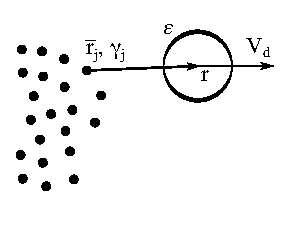
\includegraphics{VortexDiff.pdf}}
\end{center}

%%%%%%%%%%%%%%%%%%%%%%%%%%%%%%%%%%%%%%%%%%%%%%%%%%%%%%%%%%%%%%%%%%%%%%%%%%%%%%%%
\subsection{Body diffusive}

$\br r$ - координаты текущего вихря (для которого вычисляем скорость) \\
$\br W_d$ - диффузионная скорость текущего вихря, индуцированная стенкой \\
$\br p_k$ - k-я вершина тела \\
$\br r_k = \frac{1}{2}(\br p_k + \br p_{k+1})$ - центр k-го отрезка тела \\
$d \br S_k = \br n \cdot\lvert\br p_{k+1} - \br p_k \rvert$ - нормаль к k-му отрезку, с длиной, равной длине отрезка (направление --- из тела в жидкость) \\
$\br{\rho}_k = \br r - \br r_k$ - и так понятно \\

\begin{equation*}
\br I_3 = {\sum\limits_k d\br S_k\cdot e^{-\lvert\rho_k\rvert/\varepsilon}},
%\end{equation*}
%\begin{equation*}
I_0 = {\varepsilon^2\sum\limits_k \dfrac{\lvert\rho_k\rvert /\varepsilon +1}{\rho_k^2}
\cdot(\br\rho_k \cdot d\br S_k)\cdot e^{-\lvert\rho_k\rvert/\varepsilon}},
%\end{equation*}
%\begin{equation*}
\br W_d = \dfrac{1}{\Reyn} \dfrac{\br I_3}{2\pi\varepsilon^2 - I_0}
\end{equation*}

\begin{center}\setlength\fboxsep{0pt}
\setlength\fboxrule{0.5pt}
\fbox{\input{images/BodyDiff.pdf_tex}}
\end{center}

%%%%%%%%%%%%%%%%%%%%%%%%%%%%%%%%%%%%%%%%%%%%%%%%%%%%%%%%%%%%%%%%%%%%%%%%%%%%%%%%
\subsection{Heat diffusive}

\begin{equation*}
{\br V_d}_\text{heat} = \frac {1}{\Pran}\frac{1}{\Reyn} \cdot\frac{\br I_2 + \br I_3}{I_1 - I_0}
\end{equation*}

%%%%%%%%%%%%%%%%%%%%%%%%%%%%%%%%%%%%%%%%%%%%%%%%%%%%%%%%%%%%%%%%%%%%%%%%%%%%%%%%
\subsection{Ограничения $\br V_d$ и $\varepsilon$}
В новой версии все идиотизмы исправлены, и ограничение сделано максимально понятным: $I_0$ и $\gamma_i$ должны быть одного знака, и $\lvert I_0 \rvert > 0.1 \lvert\gamma_i\rvert$. 
Для $\varepsilon$ вводится ограничение снизу $\varepsilon > \langle dS_k \rangle$

%%%%%%%%%%%%%%%%%%%%%%%%%%%%%%%%%%%%%%%%%%%%%%%%%%%%%%%%%%%%%%%%%%%%%%%%%%%%%%%%
\newpage
\section{FlowMove}
\subsection{Схема Эйлера (классика)}
\begin{equation*}\begin{split}
&\dot{\br r} = \br V (\br r, t) \\
\Rightarrow~&\br r_{i+1} = \br r_i + \br V(\br r_i, t_i) \cdot \Delta t
\end{split}\end{equation*}

\subsection{Схема Эйлера с пересчетом}
\begin{equation*}\begin{split}
&\dot{\br r} = \br V (\br r, t) \\
\Rightarrow~&\tilde{\br r}_{i+1} = \br r_i + \br V(\br r_i, t_i) \cdot \Delta t \\
\Rightarrow~&\br r_{i+1} = \br r_i + 
\frac{\br V(\br r_i, t_i) + \br V( \tilde{\br r}_{i+1}, t_{i+1})}{2}\cdot \Delta t \\
\end{split}\end{equation*}
А что бы не хранить 2 скорости (или старые координаты) для
каждой частицы, да и вообще упростить работу с модулем,
последюю формулу перепишем в виде
\begin{equation*}
\Rightarrow~\br r_{i+1} = \tilde{\br r}_{i+1} + 
\left( -\br V(\br r_i, t_i) + \br V( \tilde{\br r}_{i+1}, t_{i+1}) \right)\cdot \frac{\Delta t}{2} \\
\end{equation*}

\subsection{Последовательность действий}
\begin{packed_enum}
\item ГУ не выполнены\\
\item Строим дерево
\item Берем скорости набегающего потока итд, заполняем СЛАУ
\item Решаем СЛАУ
\item Удаляем дерево\\
\item Сохраняемся: вихри, тела
\item Спускаем вихри, чернила, тепло
\item Сохраняем файл stepdata\\
\item Строим дерево
\item Считаем эпсилоны, объединяем вихри
\item Считаем скорости: Convective, Diffusive, Boundary; скорости чернил, тепла
\subitem Опционально: двигаем на пол шага, заменяем скорости на отрицательные.
\subitem Опционально: считаем вторую половину скоростей.
\item Двигаем вихри, тела, стриклайны; удаляем проникшие внутрь.
\item $t += \Delta t$
\end{packed_enum}

%%%%%%%%%%%%%%%%%%%%%%%%%%%%%%%%%%%%%%%%%%%%%%%%%%%%%%%%%%%%%%%%%%%%%%%%%%%%%%%%
\newpage
\section{Устойчивость и выбор параметров расчета}
Согласно статье в ЖВМ, параметры расчета выбираются исходя из
соображений устойчивости. Параметрами, которые мы можем менять, являются:
$N$ --- число отрезков разбиения контура;\\
$\varepsilon_{min}$ --- ограничение на эпсилон из диффузии;\\
$\Delta t$ --- шаг по времени;\\
$r_d$ --- радиус дискретности, он же эпсилон в конвективной скорости.\\

Дополнительные обозначения:\\
$\Delta l_i$ --- длина i-го отрезка на теле, соответственно \\
$\langle\Delta l \rangle=\dfrac{1}{N} \sum\limits_{i=0}^{N} \Delta l_i$ ---
средняя длина отрезков.\\
$N$ обычно выбирается на глаз.\\
$\varepsilon_{min}=0.6\cdot\langle\Delta l \rangle$ --- 
определено в модуле diffmergefast\\
$\Delta t = \Reyn \varepsilon_{min}^2 < 2 \Reyn \varepsilon^2$\\
$r_d = ?$ --- а этот вопрос остается открытым \\

\subsection{Схемная вязкость}
\begin{equation*}
\nu_\text{сх}^I = 0.018 \cdot \Omega_0^2 r_*^2 \Delta t
\end{equation*}
\begin{equation*}
\nu_\text{сх}^{II} = 5\cdot10^{-4} \cdot \dfrac{\gamma_*^2 a}{r_d^3} \cdot \Delta t
\end{equation*}

Обозначения:\\
$r_*$ --- характерный размер вихря (диаметр)\\
$\Omega_0 = \dfrac{\sum\gamma_i}{\pi r_*^2}$ --- характерная завихренность\\
$\gamma_* = \langle \gamma_i \rangle$ --- средняя циркуляция доменов\\
$a = \sqrt{\pi r_*^2 / N} $ --- характерное расстояние между доменами\\
$r_d$ --- радиус дискретности\\

%%%%%%%%%%%%%%%%%%%%%%%%%%%%%%%%%%%%%%%%%%%%%%%%%%%%%%%%%%%%%%%%%%%%%%%%%%%%%%%%
\newpage
\section{Сохранение результатов}

\subsection{Бинарники с каждого шага}
Первые 1024 байта --- закладки. Каждая закладка 16 байт. 8 байт --- название (восемь букв, и еще 8 --- указатель (номер байта в файле).\\
``Header  '' --- Общая инфа о режиме, задаваемая из мейн файла. И после этого последовотельно по 8 байт $\Delta t$, $1/\nu$, $V_{x\infty}$, $V_{y\infty}$, real time (timet), T.\\
``Vortexes'', ``Heat    '', ``StrkSrc '', ``Streak  '', ``Body    '' --- различные списки. У каждого списка первые 8 байт занимает количество элементов $N$. Оставшиеся $8\cdot 3 \cdot N$ байт уходят на массив троек ($r_x$, $r_y$, g). У списка ``Body    '' последней тройкой хранится (RotAxis.rx, RotAxis.ry, $\omega$)


\subsection{Профили трения, давления, и теплоотдачи}
Первые $2 \cdot 4$байта --- TValues, N.\\
TValues --- это enum. $C_p=1$, $Fr=2$, $Nu=4$.\\
N --- число отрезков на всех телах.\\
На каждом временном шаге сохраняется сначала текущее время (4 байта). Далее идут группы по 3--5 floatов: ($r_x$, $r_y$, [$C_p$], [$Fr$], [$Nu$])

\end{document}
